\documentclass{nature}
%\documentclass{natureprintstyle} % two column
%\documentclass{nature_submit} % With figures removed

\usepackage{graphicx}

% Simple macros
\newcommand{\bra}[1]{\langle #1|}
\newcommand{\ket}[1]{|#1\rangle}
\newcommand{\braket}[2]{\langle #1|#2\rangle}
\def\ex{{\mathbf e}_x}                            % e_x
\def\ey{{\mathbf e}_y}                            % e_y
\def\ez{{\mathbf e}_z}                            % e_z
\def\es{{\mathbf e}_s}                            % e_s
\def\nm{{\ {\rm nm}}}						% nm
\def\Rb87{^{87}\rm{Rb}}					% Rb 87
\def\Hz{{\ {\rm Hz}}}						% Hz
\def\MHz{{\ {\rm MHz}}}						% MHz
\def\ms{{\ {\rm ms}}}						% ms
\def\us{{\ \mu{\rm s}}}						% us
\def\uK{{\ \mu{\rm K}}}                                                         % uK
\def\nK{{\ {\rm nK}}}						% nK

\bibliographystyle{naturemag}
%\title{Impurity driven diffusion and destruction of solitons in quasi-1D Bose-Einstein condensates}
\title{Impurity driven Brownian motion of solitons in quasi-1D Bose-Eistein Condensates}
\author{ L. M. Aycock$^{1,2}$, H. M. Hurst$^1$,  D. Genkina$^1$, H.-I Lu$^{1}$, I. B. Spielman$^1$}
\begin{document}
\maketitle
\begin{affiliations}
 \item Joint Quantum Institute, National Institute of Standards and Technology, and University of Maryland, Gaithersburg, Maryland, 20899, USA
 \item Cornell University, Ithaca, New York, 14850, USA
\end{affiliations}

\begin{abstract}
Here, we report on the effect of evenly distributed impurity atoms on soliton dynamics. We launch lone, long-lived solitons in highly elongated $\Rb87$ Bose-Einstein condensates (BECs) by phase imprinting and observe oscillations stable over many seconds. We compare these long-lived solitons to those launched in BECs containing a few percent of impurity---the same atomic species in a different Zeeman sublevel---controllably introduced just before evaporation to degeneracy. These impurities---evenly distributed throughout the condensate---dramatically decrease the soliton lifetime and enhance Brownian-like diffusion in the soliton's trajectory.
\end{abstract}

Current experimental research on solitons focuses on their collisions with each other\cite{Becker2013,Weller2008} and how dimensionality influences their stability and decay\cite{Ku2014}.
\section{Dark long-lived solitons in BECs}
First we begin by studying long-lived, lone solitons in quasi-one-dimensional (quasi-1D) BECs. We create BECs on our previously described apparatus\cite{Lin2009e}. However, one beam of our crossed dipole beam trap is spatially modulated by modulating the frequency on an acoustic-optic modulator to create a time averaged potential. We prepare the atoms in the $\ket{F=1,m_{F}=0}$ sublevel and evaporate down to optical trap frequencies $\omega_{radial},\omega_{axial} = 2 \pi (115, 3.7)\Hz$ and a temperature of $<10\nK$. We have about $8 \times 10^{5}$ atoms and a 1-D spead of sound $\bar{c}_{s}=1.6 \rm{mm/s}$ \cite{Zaremba1998,Stringari1998,Kavoulakis1998,Andrews1997b}. Then we use typical phase imprinting techniques\cite{Burger1999,Denschlag2000} to create dark, long-lived solitons and observe their osciallations in the trap as a function of time after the phase imprint. We turn off the optical dipole potential and allow the atoms to expand. The soliton also expands from the size of the healing length to a larger density depletion easily resolved by our imaging system. We then vary the time after the phase imprint and observe oscillations as shown in Fig. \ref{solOsc}a. Each absorption image of the elongated condensate represents a singe iteration of the experiement. We vary the time after the phase imprint from 0.002 s to 4.007s. After the phase imprint, several excitations are created which include density waves, nonstationary kinks and a lone proper dark soliton \cite{Muryshev2002}. After a few hundred miliseconds, the additional excitations dissapate and tracking the position of the lone proper dark soliton becomes trivial. The non-ending soliton trajectory is traced back to small times after the phase imprint. 
\begin{figure}[h!]
   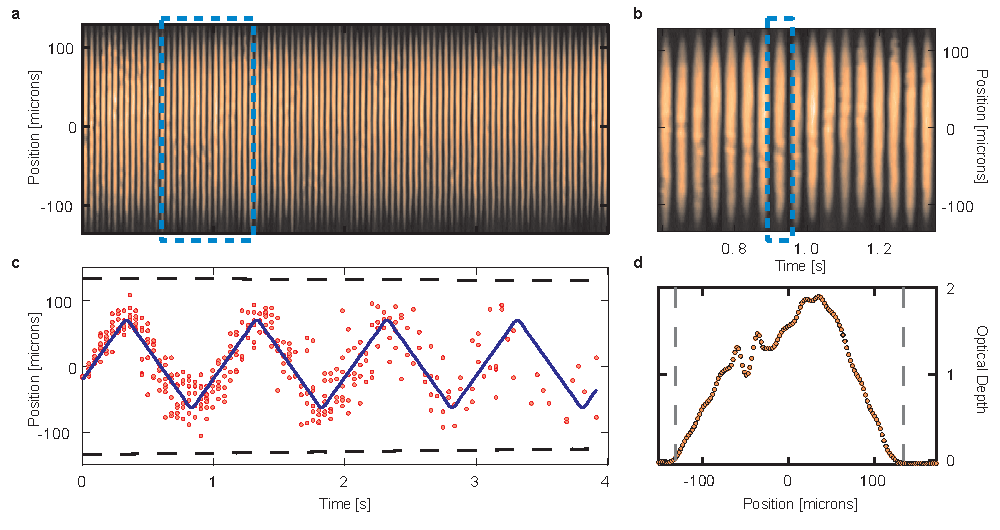
\includegraphics[width=136mm]{Figures/Fig1_solOscV3.pdf}
   \caption{\textbf{Soliton Oscillations} \textbf{a}, Individual absorbtion images of quasi-1D condensate with soliton vs time after phase imprint. Blue dashed line shows where \textbf{b} is a subset of the data. \textbf{c}, the soliton position vs time after phase imprint. Grey dashed lines represent the edges of the quasi 1-D condensate. \textbf{d} averaged density profile of the condensate in the axial direction at 0.947s after phase imprint.}
   \label{solOsc}
\end{figure}
Figure \ref{solOsc} b is magnified view of a few of the images in Fig. \ref{solOsc}a. This shows the constrast of the density depletion of the soliton. Figure \ref{solOsc} d is a 1-D density profile integrated over the two radial directions at 0.947 s after the phase imprint. The soliton has about 32\% contrast with the surrounding density profile. The minimum of the density depletion is the soliton position which is plotted in Fig. \ref{solOsc} c. For every time after the phase imrpint, there were approximately 5 images taken. The decreased number of points past 2.5 s is reflective of a decreased number of experiemental iterations with a proper dark soliton at that time after the phase imprint. The triangular shape of the osciallations is due to the flat bottomed potential the atoms experience due to the time averaged potential of dithering a Gaussian 1064nm laser beam. The fit to a Taylor series expanded triangle wave to the fifth order uses a Levenberg-Marquardt least-squares method. We will use this method for all of our data. 


\section{Methods}
Now that we have established the procedure to create lone, long-lived solitons, we now ask the impact that magnetic impurities in the $\ket{F=1,m_{F}=0}$ sublevel have on the lifetime and position trajectory of the soliton. To inject these impuriites and perform the experiments at equilibrium, we use an oscillating rf magnetic field to control the spin mixture of a thermal gas before evaporating completely to degeneracy. We intialized the thermal gas in $\ket{F=1,m_{F}=0}$ sublevel, then apply the rf magnetic field as a blackman pulse with varying amplitudes to controlably adjust the number of impruity atoms after evaporation. The percent of impurity atoms before evaporation do not directly correspond to the percent of impurity atoms at the end of evaporation due to increased evaporation efficiency in the prescence of impurities \cite{Fang2015}. 
\begin{figure}[h!]
   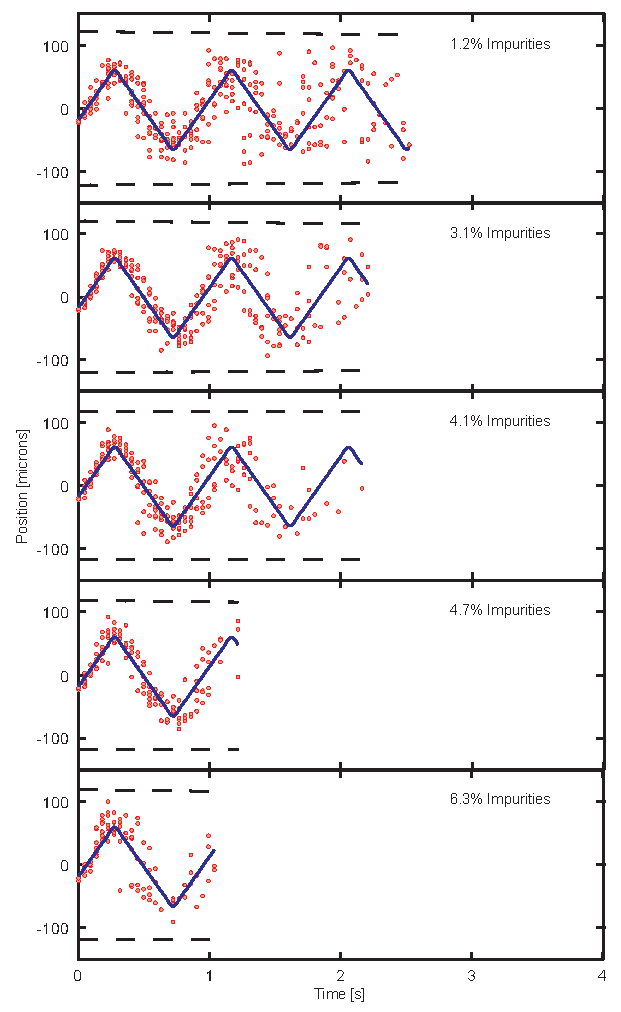
\includegraphics[width=89mm]{Figures/Fig2_solWImp.pdf}
   \caption{\textbf{Soliton Oscillations in the Presence of Impurities} Here, we plot the soliton position vs time after phase imprint for different impurity levels. The blue solid line is a global fit to all the data. The grey dashed lines represent the extent of the condensate on either end vs time.}
   \label{solWImp}
\end{figure}
\section{Impurities impact on soliton lifetime}
\begin{figure}[h!]
   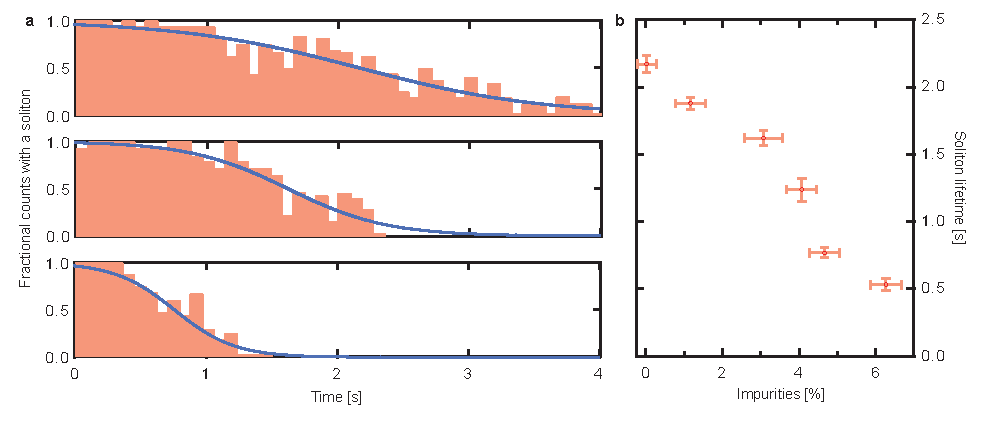
\includegraphics[width=136mm]{Figures/Fig3_Life.pdf}
   \caption{\textbf{Soliton Lifetime in the Presence of Impurities} \textbf{a}, Histograms of fractional count of data with solitons vs time after phase imprint. The blue solid line is a fit to a fermi dirac distrubution from which we extract a width and a lifetime. \textbf{b}, The lifetime extrtacted from fits of the histograms of the fractional counts with solitons vs percent impurities in the condensate.}
   \label{solLife}
\end{figure}
\section{Impuritiy enhanced brownian motion of solitons}
\begin{figure}[h!]
   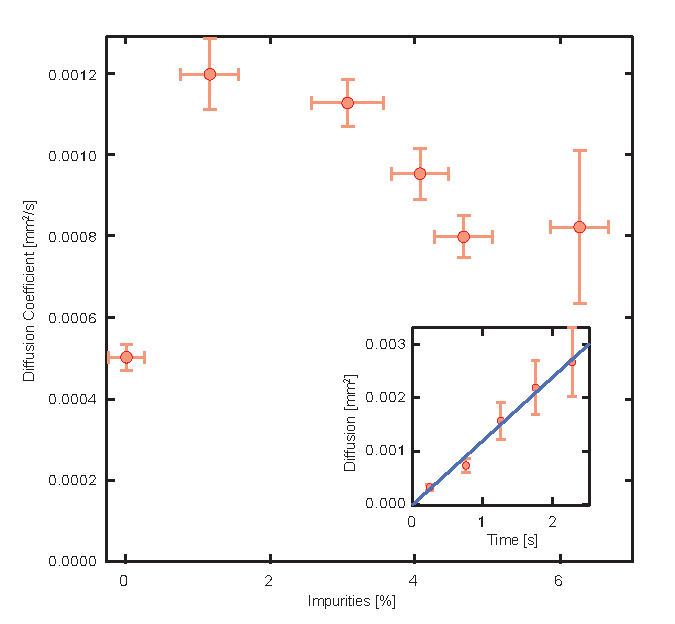
\includegraphics[width=136mm]{Figures/Fig4_Diff.pdf}
   \caption{\textbf{Browninan diffusion constant depence on impurities} This plots the diffusion constant found from fitting the square of the residuals of the fit for the soliton oscillations vs time after phase imprint. \textbf{Inset} The linear fit to the square of the residuals for 1.2\% impurities vs time after phase imprint. Data is binned into 0.5s bins, the uncertianty is the standard deviation in each bin divided by $\sqrt{N}$, where $N$ is the number of points in each bin.}
   \label{solDiff}
\end{figure}

\bibliography{library}

\begin{addendum}
\item This work was partially supported by the ARO's Atomtronics MURI, by the AFOSR's Quantum Matter MURI, NIST, and the NSF through the PFC at the JQI.

\item[Author Contributions] 

\item[Competing Interests]  The authors declare that they have no competing financial interests.

\item[Correspondence] Correspondence and requests for materials should be addressed to I.B.S. (email: ian.spielman@nist.gov).

\end{addendum}


\end{document}